% 正方形性质总图：四边相等 + 四角直角 + 对角线相等垂直平分 + 平分对角 45°
\documentclass[tikz,border=4pt]{standalone}
\usepackage{ctex}
\usepackage{amsmath}
\usetikzlibrary{calc, angles, quotes, decorations.markings, arrows.meta}
\begin{document}
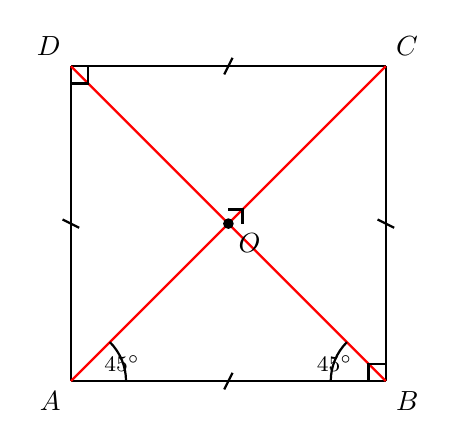
\begin{tikzpicture}[
  scale=1.0, thick,
  tickone/.style={postaction={decorate, decoration={markings,
    mark=at position 0.5 with {\draw (-1.5pt,-3pt) -- (1.5pt,3pt);}}}},
]
  \coordinate (A) at (0,0);
  \coordinate (B) at (4,0);
  \coordinate (C) at (4,4);
  \coordinate (D) at (0,4);
  \coordinate (O) at (2,2);

  % 四边（单划标记等长）
  \draw[tickone] (A) -- (B);
  \draw[tickone] (B) -- (C);
  \draw[tickone] (C) -- (D);
  \draw[tickone] (D) -- (A);

  % 对角线
  \draw[red] (A) -- (C);
  \draw[red] (B) -- (D);

  % 中心
  \filldraw (O) circle (1.5pt);

  % 右下角直角小方块
  \draw (B) ++(-0.22,0) -- ++(0,0.22) -- ++(0.22,0);
  % 左上角直角小方块
  \draw (D) ++(0.22,0) -- ++(0,-0.22) -- ++(-0.22,0);

  % 中心垂直小方块
  \draw (O) ++(0.18,0) -- ++(0,0.18) -- ++(-0.18,0);

  % 45° 角弧（A 处对角线 AC 与边 AB 的夹角）
  \draw (0.7,0) arc[start angle=0, end angle=45, radius=0.7];
  \node at (0.65,0.22) {\footnotesize $45^\circ$};
  % B 处对角线 BD 与边 BA 的 45°
  \draw (4-0.7,0) arc[start angle=180, end angle=135, radius=0.7];
  \node at (4-0.65,0.22) {\footnotesize $45^\circ$};

  \node[below left]  at (A) {$A$};
  \node[below right] at (B) {$B$};
  \node[above right] at (C) {$C$};
  \node[above left]  at (D) {$D$};
  \node[below right] at (O) {$O$};
\end{tikzpicture}
\end{document}
